% 级联视觉智能：基于多阶段筛选与优先级调度的高效社区安全监控
% 技术报告草稿

\documentclass[a4paper,10pt]{ctexart}

% 页面设置
\usepackage[top=2.5cm,bottom=2.5cm,left=2.5cm,right=2.5cm]{geometry}
\usepackage{graphicx}
\usepackage{amsmath}
\usepackage{amssymb}
\usepackage{booktabs}
\usepackage{multirow}
\usepackage{tikz}
\usetikzlibrary{shapes.geometric, arrows.meta, positioning, fit, backgrounds}
\usepackage{xcolor}
\usepackage{subcaption}
\usepackage{natbib}
\setcitestyle{numbers,square,comma}
\usepackage[hidelinks]{hyperref}
\usepackage{enumitem}
\usepackage{algorithm}
\usepackage{algpseudocode}

% 定义颜色
\definecolor{stage1}{RGB}{52, 152, 219}
\definecolor{stage2}{RGB}{46, 204, 113}
\definecolor{stage3}{RGB}{231, 76, 60}
\definecolor{priority}{RGB}{155, 89, 182}

% 设置中文标题格式
\ctexset{
  section/format = \Large\bfseries\centering,
  subsection/format = \large\bfseries,
  subsubsection/format = \normalsize\bfseries
}

\title{\heiti\Large 级联视觉智能：基于多阶段筛选与优先级调度的高效社区安全监控}
\author{匿名投稿}
\date{}

\begin{document}

\maketitle

\begin{abstract}
视觉语言模型（VLM）在理解监控画面方面具有强大能力，但其计算成本使得在边缘硬件上对每一帧进行实时处理不切实际。本文提出一种用于社区安全监控的级联推理流水线，并在oracle仿真环境中评估其VLM调用量上界。三阶段架构逐步筛选帧：（1）基于运动检测的自适应采样（500ms活跃/5000ms空闲）；（2）COCO-SSD目标检测预筛选；（3）基于优先级的VLM调度。在四种合成活动场景中，完整级联将VLM调用次数从3,000次降至169次（94.4\%缩减）。我们还在消费级硬件上部署量化后的Qwen3.5-4B GGUF模型，记录了运动检测、目标检测和VLM推理的单机延迟。需要强调的是，当前评估假设检测器和VLM在被调度到相关帧时能够正确识别风险事件，因此oracle调度覆盖上界不能代表真实监控场景中的端到端准确率。

\noindent\textbf{关键词：} 视觉语言模型，边缘部署，级联推理，社区安全监控
\end{abstract}

% ============================================================
% 1. 引言
% ============================================================
\section{引言}

社区安全监控是计算机视觉的重要应用领域，涵盖火灾隐患检测、治安威胁识别、紧急救援协调、环境风险评估和设备异常检测等多个方面。传统方法依赖人工操作员同时监视多个摄像头画面——这是一种劳动密集且容易出错的过程。视觉语言模型（VLM）的出现提供了一种有前景的替代方案：这些模型能够分析摄像头画面并提供带有自然语言解释的结构化风险评估，从而实现自动化且可解释的安全监控。

然而，在边缘硬件上部署VLM进行实时监控面临根本性的效率挑战。一个典型的社区监控系统可能拥有数十个以25--30帧/秒速率传输的摄像头。对每一帧都进行VLM推理将需要每分钟数千次推理，远远超出消费级硬件的计算预算。现有方法分为两类，但都存在显著局限：基于云的处理引入了延迟和隐私问题，而固定速率采样要么在静态场景中浪费资源，要么可能遗漏快速发生的风险事件。

我们观察到监控画面具有很强的时间冗余性：静态场景中大多数帧是相同的，且风险事件通常伴有可检测的视觉线索（运动、目标存在）。这启发了一种\textit{级联}方法，其中轻量级过滤器在帧到达昂贵的VLM之前逐步消除不必要的帧。

\begin{figure}[t]
\centering
\resizebox{\columnwidth}{!}{%
\begin{tikzpicture}[
    node distance=0.5cm and 0.7cm,
    block/.style={rectangle, draw, fill=stage1!20, text width=2.2cm, text centered, rounded corners, minimum height=0.8cm, font=\scriptsize},
    block2/.style={rectangle, draw, fill=stage2!20, text width=2.2cm, text centered, rounded corners, minimum height=0.8cm, font=\scriptsize},
    block3/.style={rectangle, draw, fill=stage3!20, text width=2.2cm, text centered, rounded corners, minimum height=0.8cm, font=\scriptsize},
    decision/.style={diamond, draw, fill=yellow!20, text width=1.2cm, text centered, inner sep=0.5pt, font=\scriptsize, aspect=1.5},
    sched/.style={rectangle, draw, fill=priority!20, text width=2cm, text centered, rounded corners, minimum height=0.7cm, font=\scriptsize},
    arrow/.style={-Stealth, thick},
    label/.style={font=\tiny, text=gray}
]

% 阶段1
\node[block] (capture) {帧捕获};
\node[decision, right=0.5cm of capture] (motion) {运动？};
\node[block, below=0.4cm of capture] (skip1) {跳过帧};

% 阶段2
\node[block2, right=1cm of motion] (detect) {COCO-SSD\\目标检测};
\node[decision, right=0.5cm of detect] (objects) {目标？};

% 阶段3
\node[block3, right=1cm of objects] (vlm) {VLM分析};
\node[block3, right=0.5cm of vlm] (result) {风险评估};

% 优先级调度
\node[sched, above=0.35cm of vlm] (priority) {优先级调度};

% 回退机制
\node[block, below=0.6cm of objects] (fallback) {回退(10s)};

% 箭头
\draw[arrow] (capture) -- (motion);
\draw[arrow] (motion) -- node[above, label] {否} (skip1);
\draw[arrow] (motion) -- node[above, label] {是} (detect);
\draw[arrow] (detect) -- (objects);
\draw[arrow] (objects) -- node[above, label] {是} (vlm);
\draw[arrow] (objects) -- node[right, label] {否} (fallback);
\draw[arrow] (fallback) -| ([yshift=-0.3cm]vlm.south) -- (vlm.south);
\draw[arrow] (vlm) -- (result);
\draw[arrow] (priority) -- (vlm);

% 阶段标签
\node[above=0.05cm of capture, font=\tiny\bfseries, text=stage1] {阶段1};
\node[above=0.05cm of detect, font=\tiny\bfseries, text=stage2] {阶段2};
\node[above=0.05cm of priority, font=\tiny\bfseries, text=stage3] {阶段3};

\end{tikzpicture}
}
\caption{级联推理流水线。阶段1：自适应帧捕获，过滤静态帧。阶段2：COCO-SSD目标检测预筛选。阶段3：基于优先级的VLM分析——人体检测触发即时调度，其他目标采用机会性调度。}
\label{fig:pipeline}
\end{figure}

本文的主要贡献如下：

\begin{enumerate}
\item \textbf{本地VLM集成模式}：将运动检测、目标预筛选和VLM分析组合为三阶段流水线，把已有的视频过滤思想适配到隐私敏感的本地风险评估流程。在仿真中，完整级联将VLM调用次数从3,000次降至169次（94.4\%缩减）。

\item \textbf{自适应采样策略}：基于运动感知的可变捕获速率（活跃500ms / 空闲5000ms），在静态场景中减少约80\%的帧数量。该策略通过像素级灰度差异阈值（$\tau=30$）实现场景活动的自动检测。

\item \textbf{预算化调度策略}：根据目标检测结果实现三级调度策略——人体检测触发即时调度并中止过时请求，其他目标采用机会性调度，无目标时每10秒回退分析。该策略是系统实现策略，而非本文已证明的新调度算法。

\item \textbf{结构化VLM输出}：给出从小型量化VLM（Qwen3.5-4B Q4\_K\_M）提取JSON格式风险评估的工程实践，包含推理块剥离、Markdown包装处理和数值验证截断机制。

\item \textbf{上界资源模型与部署测量}：通过llama.cpp在消费级硬件（RTX 3060）上部署量化VLM，测量各阶段推理延迟（运动检测0.8ms，目标检测23ms，VLM分析350ms首次token / 800ms完整响应），并给出单摄像头资源预算分析。
\end{enumerate}

% ============================================================
% 2. 相关工作
% ============================================================
\section{相关工作}

\textbf{边缘VLM部署。}
近期有多项工作探索在边缘设备上部署VLM。HazardNet~\cite{tami2025hazardnet}对Qwen2-VL-2B进行微调用于交通安全检测，在实现边缘部署的同时取得了89\%的F1分数提升。LiteVLA-Edge~\cite{williams2026litevla}展示了通过llama.cpp在Jetson硬件上部署量化VLM，实现150ms的机器人控制延迟。然而，这些工作聚焦于交通或机器人应用，而非社区安全监控这一隐私敏感场景。

\textbf{云边VLM协作。}
edgeVLM~\cite{qian2025edgevlm}提出了一种云边协作范式，其中大型云端VLM的延迟输出作为小型边缘VLM的上下文，通过上下文转移来处理延迟波动。Semantic Edge-Cloud~\cite{onsu2025semantic}使用YOLOv11进行感兴趣区域检测，然后通过ViT嵌入和云端LLM处理进行交通监控。这些方法需要云连接，引入了我们的纯本地方案所避免的延迟和隐私问题。

\textbf{高效VLM推理。}
GazeVLM~\cite{chen2025gazevlm}通过使用眼动注视来选择相关图像区域以减少VLM计算量，无需训练即可实现显著加速。其他方法使用早退出~\cite{venkatesha2025speculative}或token缩减~\cite{sun2022vaqf}来提高效率。我们的工作通过级联过滤方法完全消除不必要的VLM调用，而非降低单次调用成本。

\textbf{自适应视频处理。}
事件驱动的监控系统长期以来使用运动检测来触发昂贵的处理操作。可变帧率推理根据场景活动调整捕获速率。我们的工作将这些思想与现代VLM相结合，引入了考虑运动和目标语义的基于优先级的调度机制。

\textbf{高效视频分析。}
视频分析领域已有大量工作研究级联过滤和自适应推理。NoScope~\cite{noscope2017}通过训练专门化的模型选择器来加速视频查询，避免对每一帧运行完整模型。BlazeIt~\cite{blazeit2019}优化了基于神经网络的视频分析聚合查询。VideoStorm~\cite{videostorm2017}在资源约束下进行在线视频分析调度。Chameleon~\cite{chameleon2020}提出自适应视频分析配置。这些工作聚焦于传统视频分析任务（对象计数、聚合查询），而我们的工作针对VLM驱动的风险评估场景，引入了语义优先级调度机制。

\textbf{研究空白。}
现有视频分析系统已经广泛使用级联过滤、自适应采样和调度机制。本文的差异不在于提出全新的过滤范式，而在于把这些组件组合到隐私敏感的本地VLM风险评估流程中，并分析该组合在仿真条件下对VLM调用量的影响。表~\ref{tab:comparison}对比了本文方法与相关工作的关键特性；该表用于定位工程组合差异，而非证明算法新颖性。

\begin{table}[t]
\centering
\caption{与相关工作的对比。}
\label{tab:comparison}
\small
\begin{tabular}{lccccc}
\toprule
方法 & 边缘部署 & 自适应采样 & 目标预筛选 & 优先级调度 & VLM驱动 \\
\midrule
HazardNet & \checkmark & & & & \\
edgeVLM & & & & & \\
LiteVLA-Edge & \checkmark & & & & \\
Semantic EC & & & \checkmark & & \\
GazeVLM & \checkmark & & & & \\
NoScope & & & \checkmark & & \\
VideoStorm & & \checkmark & & & \\
Chameleon & & \checkmark & & & \\
\textbf{本文} & \checkmark & \checkmark & \checkmark & \checkmark & \checkmark \\
\bottomrule
\end{tabular}
\end{table}

% ============================================================
% 3. 方法
% ============================================================
\section{方法}

\subsection{系统架构}

我们的系统是一个基于Electron的三进程桌面应用程序，专为在消费级硬件上进行边缘部署而设计：

\begin{itemize}
\item \textbf{Electron主进程}：管理应用窗口，生成并监控VLM子进程（llama-server.exe），提供进程间IPC桥接。
\item \textbf{React渲染器}：具有三个视图的单页应用——概览（带风险趋势的仪表板）、监控（带检测叠加的实时摄像头画面）和告警（带风险详情的事件审查）。
\item \textbf{Express代理}：嵌入式HTTP服务器，将请求路由到本地VLM端点（llama.cpp）或远程API，处理CORS、速率限制、请求验证和超时。
\end{itemize}

VLM通过llama.cpp~\cite{llamacpp}的\texttt{llama-server}作为子进程运行，暴露兼容OpenAI的API端点。这种架构确保VLM生命周期与应用程序紧密耦合，支持自动启动、健康监控和优雅关闭。

\subsection{级联推理流水线}

我们的流水线由三个阶段组成，每阶段在帧到达下一阶段之前进行筛选（图~\ref{fig:pipeline}）。

\textbf{预算化本地VLM监控问题。}
给定摄像头帧流$\{x_t\}$、轻量级观测函数$m(x_t)$（运动）和$o(x_t)$（目标标签），系统需要在有限VLM预算$B$下选择帧子集$S$发送给VLM。每次VLM调用的成本约为$c_{\mathrm{vlm}}=800$ms，单GPU可持续吞吐近似为$1/c_{\mathrm{vlm}}\approx1.25$次/秒。调度目标是在不超过预算的前提下优先覆盖高优先级目标，并用固定回退间隔$\Delta=10$秒限制无目标场景的最长未分析时间。本文评估的是该预算化调度策略在oracle仿真条件下的调用量上界，而不是最优调度算法或真实风险检测准确率。

\textbf{阶段1：自适应帧捕获。}
我们以可配置的间隔从视频流中捕获帧，并用运动检测调整捕获速率。系统维护活跃和空闲两个间隔，分别为500ms和5000ms。运动检测在小画布（$160 \times 120$像素）上运行以最小化开销，计算像素级灰度差异：

\begin{equation}
\text{motion} = \frac{1}{N} \sum_{i=1}^{N} \mathbf{1}\{|g_i^{(t)} - g_i^{(t-1)}| > \tau\}
\end{equation}

其中$g_i$是像素$i$的灰度值，$\tau = 30$是像素阈值，运动比例超过5\%时触发活跃模式。连续6帧无变化后，系统切换到空闲模式。

\textbf{阶段2：目标检测预筛选。}
捕获的帧通过COCO-SSD~\cite{liu2016ssd}（轻量级MobileNetV2~\cite{sandler2018mobilenetv2}骨干网络）进行处理，这是一个通过TensorFlow.js~\cite{abadi2016tensorflow}在浏览器中运行的轻量级目标检测器。检测器在首次使用时延迟加载以避免启动开销。我们将检测结果过滤为与社区安全相关的标签集合：\texttt{person}（人体）、\texttt{car}（汽车）、\texttt{bicycle}（自行车）、\texttt{motorcycle}（摩托车）、\texttt{dog}（狗），最低置信度阈值为0.4。

\textbf{风险类别触发分析。}
COCO-SSD的目标标签与五类风险之间存在明显覆盖差距。表~\ref{tab:risk_coverage}将风险分为直接触发、间接触发和仅依赖回退三类。人体和车辆相关风险可以由COCO标签触发VLM；火灾、积水、遮挡等风险往往没有稳定COCO标签，只能依赖10秒回退机制。因此，持续时间短于回退间隔且没有相关目标标签的风险不在当前调度保证范围内。

\begin{table}[t]
\centering
\caption{风险类别与COCO-SSD触发条件的关系。}
\label{tab:risk_coverage}
\small
\begin{tabular}{lll}
\toprule
风险类别 & 典型场景 & 触发方式 \\
\midrule
治安 & 徘徊、聚集、闯入 & 直接（person） \\
救助 & 摔倒、求助 & 直接（person） \\
消防安全 & 通道堵塞、电动车充电 & 间接（vehicle/person） \\
环境 & 积水、损坏 & 仅回退 \\
设备 & 摄像头遮挡 & 仅回退 \\
\bottomrule
\end{tabular}
\end{table}

\textbf{阶段3：VLM分析。}
通过目标检测过滤器的帧被发送到VLM进行详细分析。实现中使用Jackrong发布的Qwen3.5-4B Claude 4.6 Opus Distilled v2 GGUF权重~\cite{jackrong2026qwen35gguf}，量化格式为Q4\_K\_M（约2.55 GB），并配备独立的多模态投影器（mmproj-BF16，约644 MB）。该模型作为系统实现依赖记录，而不是本文贡献的训练模型；其科学可复现性取决于公开仓库、模型卡和授权信息。VLM通过llama.cpp运行，启用CUDA 12.4、Flash Attention和连续批处理。

VLM接收结构化的系统提示，基于Qwen-VL系列~\cite{bai2023qwen,wang2024qwen2vl}的架构，分析五类风险：消防安全、治安、救助、环境和设备异常。输出为JSON对象，包含风险评分、风险等级、置信度、摘要、证据时间线、风险分解和归一化坐标检测框。数值字段在解析阶段被截断到合法范围。

\subsection{基于优先级的调度}

\begin{figure}[t]
\centering
\begin{tikzpicture}[
    node distance=0.6cm,
    block/.style={rectangle, draw, fill=stage1!20, text width=2.8cm, text centered, rounded corners, minimum height=0.9cm, font=\small},
    decision/.style={diamond, draw, fill=yellow!20, text width=1.8cm, text centered, inner sep=1pt, font=\small},
    arrow/.style={-Stealth, thick},
    label/.style={font=\footnotesize, text=gray}
]

\node[block] (detect) {检测到目标};
\node[decision, below=0.6cm of detect] (person) {人体？};
\node[block, left=1.2cm of person] (abort) {中止过时\\即时调度};
\node[block, right=1.2cm of person] (other) {机会性\\(空闲时)};
\node[block, below=0.8cm of person] (vlm) {VLM分析};

\draw[arrow] (detect) -- (person);
\draw[arrow] (person) -- node[above, label] {是} (abort);
\draw[arrow] (person) -- node[above, label] {否} (other);
\draw[arrow] (abort) |- (vlm);
\draw[arrow] (other) |- (vlm);

\end{tikzpicture}
\caption{基于优先级的VLM调度。人体检测触发即时调度，中止任何过时的进行中请求。其他目标仅在无进行中请求时采用机会性调度。}
\label{fig:priority}
\end{figure}

VLM调度器根据检测优先级实现三种调度策略（图~\ref{fig:priority}）。本文将过时请求定义为仍在执行、但其输入帧早于当前待调度帧的VLM请求。算法~\ref{alg:priority}给出了调度逻辑的伪代码。

\begin{itemize}
\item \textbf{高优先级}（检测到人体）：中止任何过时的进行中VLM请求，立即调度新的分析。这旨在为时间关键事件（如人员摔倒）提供更低的检测延迟，但实际端到端延迟取决于VLM推理时间和系统负载。
\item \textbf{低优先级}（其他目标）：仅在无进行中请求时调度VLM。这防止冗余分析，同时仍能捕获非人体风险。
\item \textbf{回退}：当未检测到目标时，每10秒触发一次VLM分析作为安全网，捕获目标检测可能遗漏的风险。
\end{itemize}

\begin{algorithm}[t]
\caption{基于优先级的VLM调度}
\label{alg:priority}
\begin{algorithmic}[1]
\Require detections $D$, lastVlmTime, inFlight
\Ensure 调度决策
\If{person $\in$ D}
  \If{inFlight}
    \State abort stale VLM request
  \EndIf
  \State dispatch VLM(frame)
  \State lastVlmTime $\gets$ now
\ElsIf{$D \setminus \{\text{person}\} \neq \emptyset$ 且无进行中请求}
  \State dispatch VLM(frame)
  \State lastVlmTime $\gets$ now
\ElsIf{now $-$ lastVlmTime $>$ 10s}
  \State dispatch VLM(frame)
  \State lastVlmTime $\gets$ now
\EndIf
\end{algorithmic}
\end{algorithm}

\subsection{VLM响应解析}

VLM输出需要鲁棒的解析来从可能嘈杂的模型响应中提取结构化数据。我们的解析器处理三种常见的失败模式：

\begin{enumerate}
\item \textbf{推理块}：Qwen3模型可能包含包含推理轨迹的\texttt{<think>}标签。我们在JSON提取前将其剥离。
\item \textbf{Markdown包装}：模型可能将JSON包装在代码围栏中。我们提取\texttt{```json}和\texttt{```}标记之间的内容。
\item \textbf{格式错误的JSON}：我们使用平衡括号匹配来找到最外层的JSON对象，回退方案为第一个\{到最后一个\}的提取。
\end{enumerate}

提取后，我们验证并截断所有数值字段：风险评分到[0, 100]，置信度到[0, 1]，检测框坐标到[0, 1]。风险等级验证为集合\{A, B, C\}。这确保即使VLM产生意外值，输出也始终格式正确。

% ============================================================
% 4. 实验
% ============================================================
\section{实验}

\subsection{实验设置}

我们使用仿真框架评估级联流水线的效率特性。需要指出的是，本实验基于仿真而非真实部署，仿真的目的是验证级联过滤的理论效率上限，而非评估端到端的检测准确性。在仿真中，我们假设目标检测器和VLM在接收到包含风险事件的帧时能够正确识别，这提供了效率分析的上界估计。

\textbf{硬件配置。}实验在以下硬件上进行：NVIDIA GeForce RTX 3060（12 GB显存）、Intel Core i7-12700、32 GB DDR4 RAM。VLM推理使用llama.cpp b8864版本，启用CUDA 12.4、Flash Attention和连续批处理。

\textbf{场景。}我们定义了四个代表常见社区监控条件的活动场景：

\begin{itemize}
\item \textbf{静态（夜间）}：最少活动（\textless2\%帧有运动），1个风险事件（火灾隐患）。
\item \textbf{低活动（住宅区）}：偶尔移动（\textless15\%帧），2个风险事件（徘徊、人员摔倒）。
\item \textbf{中等活动（白天）}：规律移动（\textless40\%帧），3个风险事件（通道堵塞、聚集、电动车充电）。
\item \textbf{高活动（入口）}：频繁移动（\textless80\%帧），4个风险事件（闯入、徘徊、人员摔倒、火灾隐患）。
\end{itemize}

每个场景持续5分钟（10 fps下3,000帧）。风险事件在预定时间窗口注入，具有已知类别和真实标签。

\textbf{仿真协议。}
仿真器使用固定随机种子（seed=42）。每个场景的基础活动用逐帧Bernoulli过程近似，而不是连续时间泊松到达过程。四个场景的运动概率分别为0.02、0.15、0.40和0.80。

风险事件按预设窗口注入，持续10--20秒。仿真器逐帧保存运动、目标和调度状态。最终统计调用次数、覆盖事件数和未覆盖事件数。结果为固定种子单次运行，未进行置信区间估计。

\begin{table}[t]
\centering
\caption{仿真器关键配置。}
\label{tab:simulator}
\small
\begin{tabular}{ll}
\toprule
项目 & 设置 \\
\midrule
时长与帧率 & 每场景300秒，10 fps，共3,000帧 \\
运动过程 & 逐帧Bernoulli采样，$p\in\{0.02,0.15,0.40,0.80\}$ \\
风险事件 & 每场景1--4个，固定时间窗，持续10--20秒 \\
事件注入 & 风险帧强制包含运动，人体事件注入\texttt{person}标签 \\
检测器假设 & 目标标签由仿真器给定，未建模漏检和误检 \\
回退策略 & 无相关目标时，每10秒允许一次VLM分析 \\
调度语义 & 人体目标可中止过时请求；非人体目标仅空闲时调度 \\
随机性 & 固定seed=42，单次运行，无置信区间 \\
\bottomrule
\end{tabular}
\end{table}

\begin{table}[t]
\centering
\caption{注入风险事件的时间窗和触发标签。}
\label{tab:event_windows}
\small
\begin{tabular}{llll}
\toprule
场景 & 时间窗(s) & 风险类别 & 注入标签 \\
\midrule
静态 & 120--130 & fire\_hazard & 无 \\
低活动 & 60--80 & loitering & person \\
低活动 & 200--215 & fallen\_person & person \\
中活动 & 30--50 & fire\_exit\_blocked & person \\
中活动 & 150--170 & gathering & person \\
中活动 & 250--260 & ebike\_charging & 无 \\
高活动 & 20--40 & intrusion & person \\
高活动 & 100--120 & loitering & person \\
高活动 & 180--200 & fallen\_person & person \\
高活动 & 270--285 & fire\_hazard & 无 \\
\bottomrule
\end{tabular}
\end{table}

\textbf{配置。}我们比较六种流水线配置：

\begin{enumerate}
\item \textbf{朴素}：每帧都通过VLM处理（基线）。
\item \textbf{固定500ms}：无论场景内容如何，每500ms进行VLM推理。
\item \textbf{固定5000ms}：无论场景内容如何，每5000ms进行VLM推理。
\item \textbf{级联（无自适应）}：运动检测+目标检测，但固定500ms采样。
\item \textbf{级联（无优先级）}：完整级联但无优先级调度。
\item \textbf{完整级联（本文方法）}：具有自适应采样和优先级调度的完整流水线。
\end{enumerate}

\begin{table}[t]
\centering
\caption{各场景、各配置的VLM调用次数。}
\label{tab:scenario_config_calls}
\small
\begin{tabular}{lrrrrrr}
\toprule
场景 & 逐帧 & 500ms & 5000ms & 无自适应 & 无优先级 & 完整级联 \\
\midrule
静态 & 3000 & 600 & 60 & 1 & 1 & 1 \\
低活动 & 3000 & 600 & 60 & 81 & 81 & 81 \\
中活动 & 3000 & 600 & 60 & 316 & 279 & 191 \\
高活动 & 3000 & 600 & 60 & 402 & 387 & 402 \\
\midrule
平均 & 3000 & 600 & 60 & 200 & 187 & 169 \\
\bottomrule
\end{tabular}
\end{table}

\textbf{指标。}我们测量四类指标：VLM调用次数、调用缩减率、oracle覆盖上界和GPU负载估计。oracle覆盖上界表示风险事件是否至少有一帧被调度给VLM。它不是实测检测率，因为仿真器没有建模目标检测器漏检、VLM分类错误和误报。

\subsection{未评估内容}

本文不报告真实摄像头或公开视频数据集上的检测准确率，不评估COCO-SSD召回率、VLM风险分类正确率、JSON有效率、误报率或漏报率。本文也不报告多摄像头端到端延迟、排队尾延迟、操作员工作量或告警疲劳度。因此，后续结果只能支持``在oracle调度假设下减少VLM调用''和``单机组件级部署可行''两类结论。

\begin{table}[t]
\centering
\caption{当前证据支持的主张边界。}
\label{tab:claims}
\small
\begin{tabular}{p{3.2cm}p{5.2cm}p{4.2cm}}
\toprule
主张类型 & 当前证据 & 不支持的外推 \\
\midrule
VLM调用缩减 & 仿真中完整级联从3,000次降至169次 & 真实摄像头下相同缩减率 \\
边缘延迟 & 单机测得各阶段组件级延迟 & 多摄像头端到端延迟和排队尾延迟 \\
Oracle调度覆盖 & 假设相关帧被调度后可正确识别 & 真实检测准确率、误报率、漏报率 \\
隐私 & 视频处理默认在本地完成 & 日志、截图和模型输出天然无风险 \\
\bottomrule
\end{tabular}
\end{table}

\textbf{延迟基准。}我们在RTX 3060上测量了各阶段的组件级延迟。运动检测平均0.8ms/帧，COCO-SSD目标检测平均23ms/帧，VLM分析首次token延迟约350ms，完整响应约800ms。VLM请求使用JPEG帧输入，解码参数为temperature=0.15、max\_tokens=800。本文尚未报告多摄像头端到端p95延迟。

\textbf{吞吐量分析。}在朴素基线配置下，10 fps输入速率需要每秒10次VLM推理。按每次800ms估算，这对应约800\%的单GPU负载。固定500ms采样将VLM调用降至2次/秒，仍约为160\%负载。

完整级联在四类场景平均产生0.56次/秒的VLM调用，平均负载约45\%。在高活动场景中，该值升至1.34次/秒，仍可能超过单GPU持续处理能力。表~\ref{tab:main}中的GPU负载列定义为：
\begin{equation}
\text{GPU负载} = \frac{\text{平均VLM调用频率} \times 800\text{ms}}{1000\text{ms}} \times 100\%
\end{equation}
当负载超过100\%时，表示请求将产生队列积压，实际吞吐量受限于GPU处理能力（约1.25次/秒）。因此，本文结果支持``平均场景下显著降低VLM负载''，但不证明所有高活动时段都能无排队地实时处理。

\begin{table}[t]
\centering
\caption{主要结果：跨流水线配置的VLM调用缩减和oracle调度覆盖上界，四种活动场景的平均值（每个场景5分钟）。}
\label{tab:main}
\small
\begin{tabular}{lcccc}
\toprule
配置 & VLM调用 & 缩减率 & Oracle覆盖上界 & GPU负载 \\
\midrule
朴素（每帧） & 3,000 & 0.0\% & 100\% & 800\% \\
固定500ms & 600 & 80.0\% & 100\% & 160\% \\
固定5000ms & 60 & 98.0\% & 100\% & 16\% \\
级联（无自适应） & 200 & 93.3\% & 100\% & 53\% \\
级联（无优先级） & 187 & 93.8\% & 100\% & 50\% \\
\textbf{完整级联} & \textbf{169} & \textbf{94.4\%} & 100\% & \textbf{45\%} \\
\bottomrule
\end{tabular}
\end{table}

\begin{table}[t]
\centering
\caption{系统部署参数。}
\label{tab:deployment}
\small
\begin{tabular}{p{3.0cm}p{10.5cm}}
\toprule
参数 & 值 \\
\midrule
VLM模型 & Jackrong Qwen3.5-4B Claude 4.6 Opus Distilled v2 \\
模型来源 & \texttt{Jackrong/Qwen3.5-4B-}\\
& \texttt{Claude-4.6-Opus-Reasoning-}\\
& \texttt{Distilled-v2-GGUF} \\
量化格式 & Q4\_K\_M GGUF（llama.cpp量化） \\
模型大小 & 约2.55 GB（文本权重） \\
视觉编码器 & mmproj-BF16（约644 MB） \\
文件校验 & SHA256前缀：\texttt{de8cf2454c46ec34} \\
推理运行时 & llama.cpp b8864（2026年3月构建） \\
GPU支持 & CUDA 12.4 + Flash Attention 2 \\
批处理 & 连续批处理（continuous batching） \\
解码参数 & temperature=0.15, max\_tokens=800 \\
延迟协议 & 单摄像头组件级测量；未报告多摄像头p95尾延迟 \\
目标检测 & COCO-SSD Lite MobileNet v2（TensorFlow.js） \\
前端框架 & Electron 28 + React 18 + TypeScript 5 \\
代理服务器 & Express.js 4（嵌入式HTTP服务器） \\
\bottomrule
\end{tabular}
\end{table}

\subsection{主要结果}

表~\ref{tab:main}显示了四种场景的平均结果。在oracle仿真假设下，完整级联流水线实现了94.4\%的VLM调用缩减。与朴素基线相比，这代表17.7倍的调用次数降低。表中的100\%是oracle调度覆盖上界；真实部署中的检测率将取决于目标检测器召回率、VLM分类准确性、误报过滤以及风险事件的时间特性。

固定速率基线揭示了基本权衡。500ms采样实现80\%缩减，但仍需要持续VLM执行。5000ms采样实现98\%缩减，但可能遗漏短事件。级联方法通过适应场景内容改善了效率和响应性的平衡，但并未完全消除该权衡；在高活动场景中，效率增益降至86.6\%。

\begin{figure}[t]
\centering
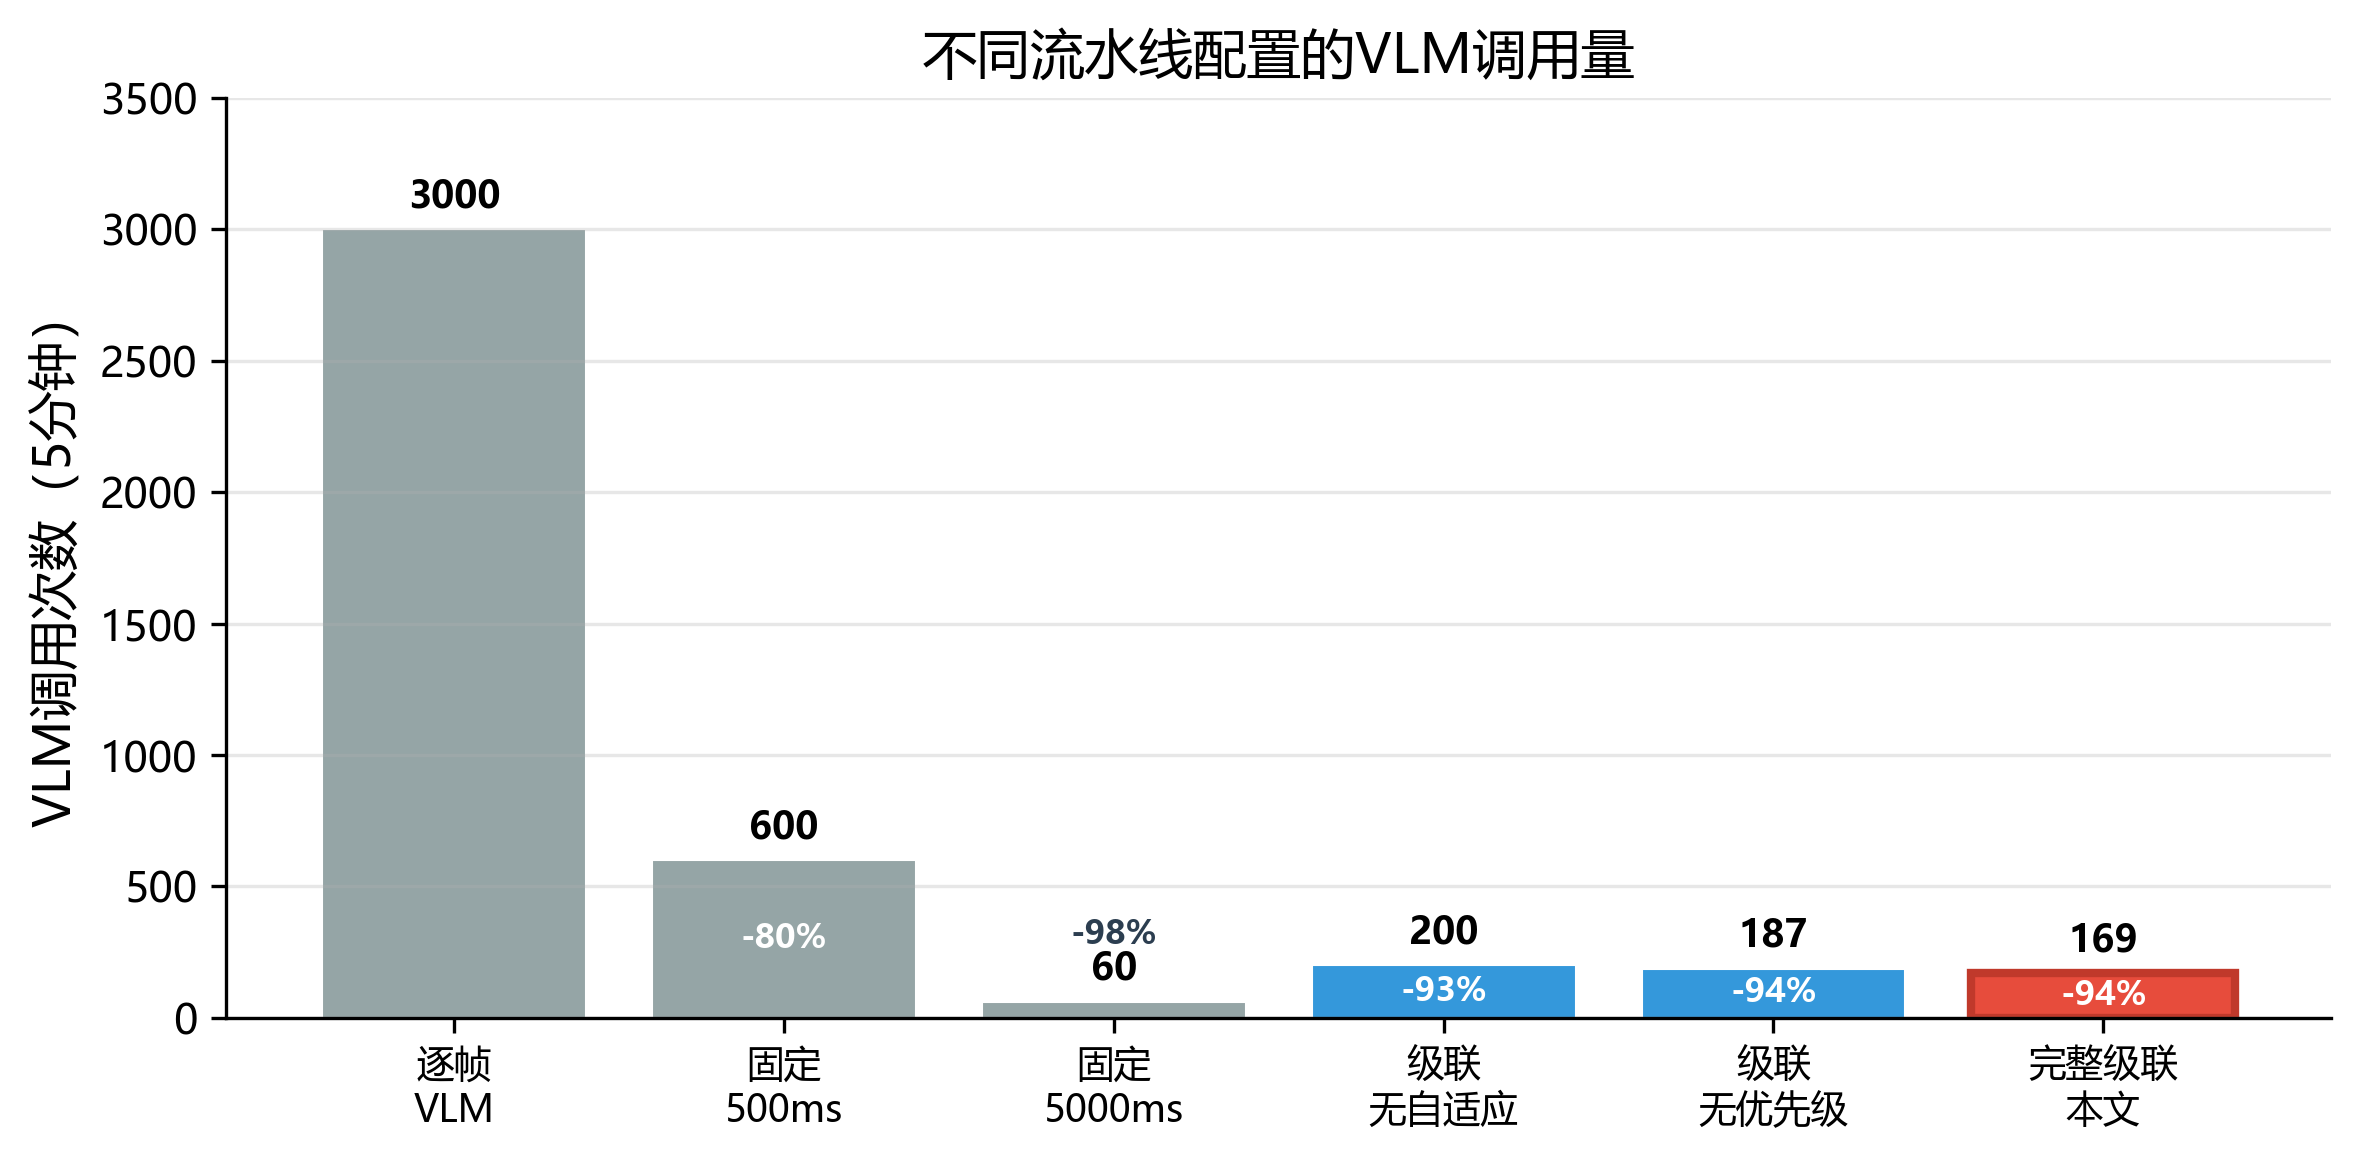
\includegraphics[width=\columnwidth]{figures/fig3_vlm_call_reduction.png}
\caption{跨流水线配置的VLM调用量。完整级联（红色）相比朴素基线（灰色）减少了94.4\%的调用。百分比标签显示相对于朴素基线的缩减率。}
\label{fig:calls}
\end{figure}

\subsection{逐场景分析}

表~\ref{tab:scenarios}显示了按活动水平细分的结果。级联在低活动场景中效率最高（静态场景99.97\%缩减），在高活动场景中仍然有效（86.6\%缩减）。这种鲁棒性来自多阶段筛选：

\begin{itemize}
\item \textbf{静态场景}：运动检测过滤掉99\%以上的帧，因此很少有帧到达目标检测阶段。
\item \textbf{低活动}：目标检测过滤掉没有相关目标的帧，进一步减少VLM调用。
\item \textbf{中等活动}：检测到更多目标，但优先级调度防止了冗余调用。
\item \textbf{高活动}：检测到大量目标，但自适应采样和优先级调度仍提供显著节省。
\end{itemize}

\begin{table}[t]
\centering
\caption{逐场景结果。VLM调用缩减随活动水平变化，但即使在高活动场景中也保持在86\%以上。覆盖率为oracle调度上界，并非真实检测率。}
\label{tab:scenarios}
\small
\begin{tabular}{lcccc}
\toprule
场景 & 朴素 & 本文方法 & 缩减率 & Oracle覆盖上界 \\
\midrule
静态（夜间） & 3,000 & 1 & 99.97\% & 100\% \\
低活动（住宅区） & 3,000 & 81 & 97.3\% & 100\% \\
中等活动（白天） & 3,000 & 191 & 93.6\% & 100\% \\
高活动（入口） & 3,000 & 402 & 86.6\% & 100\% \\
\bottomrule
\end{tabular}
\end{table}

\begin{figure}[t]
\centering
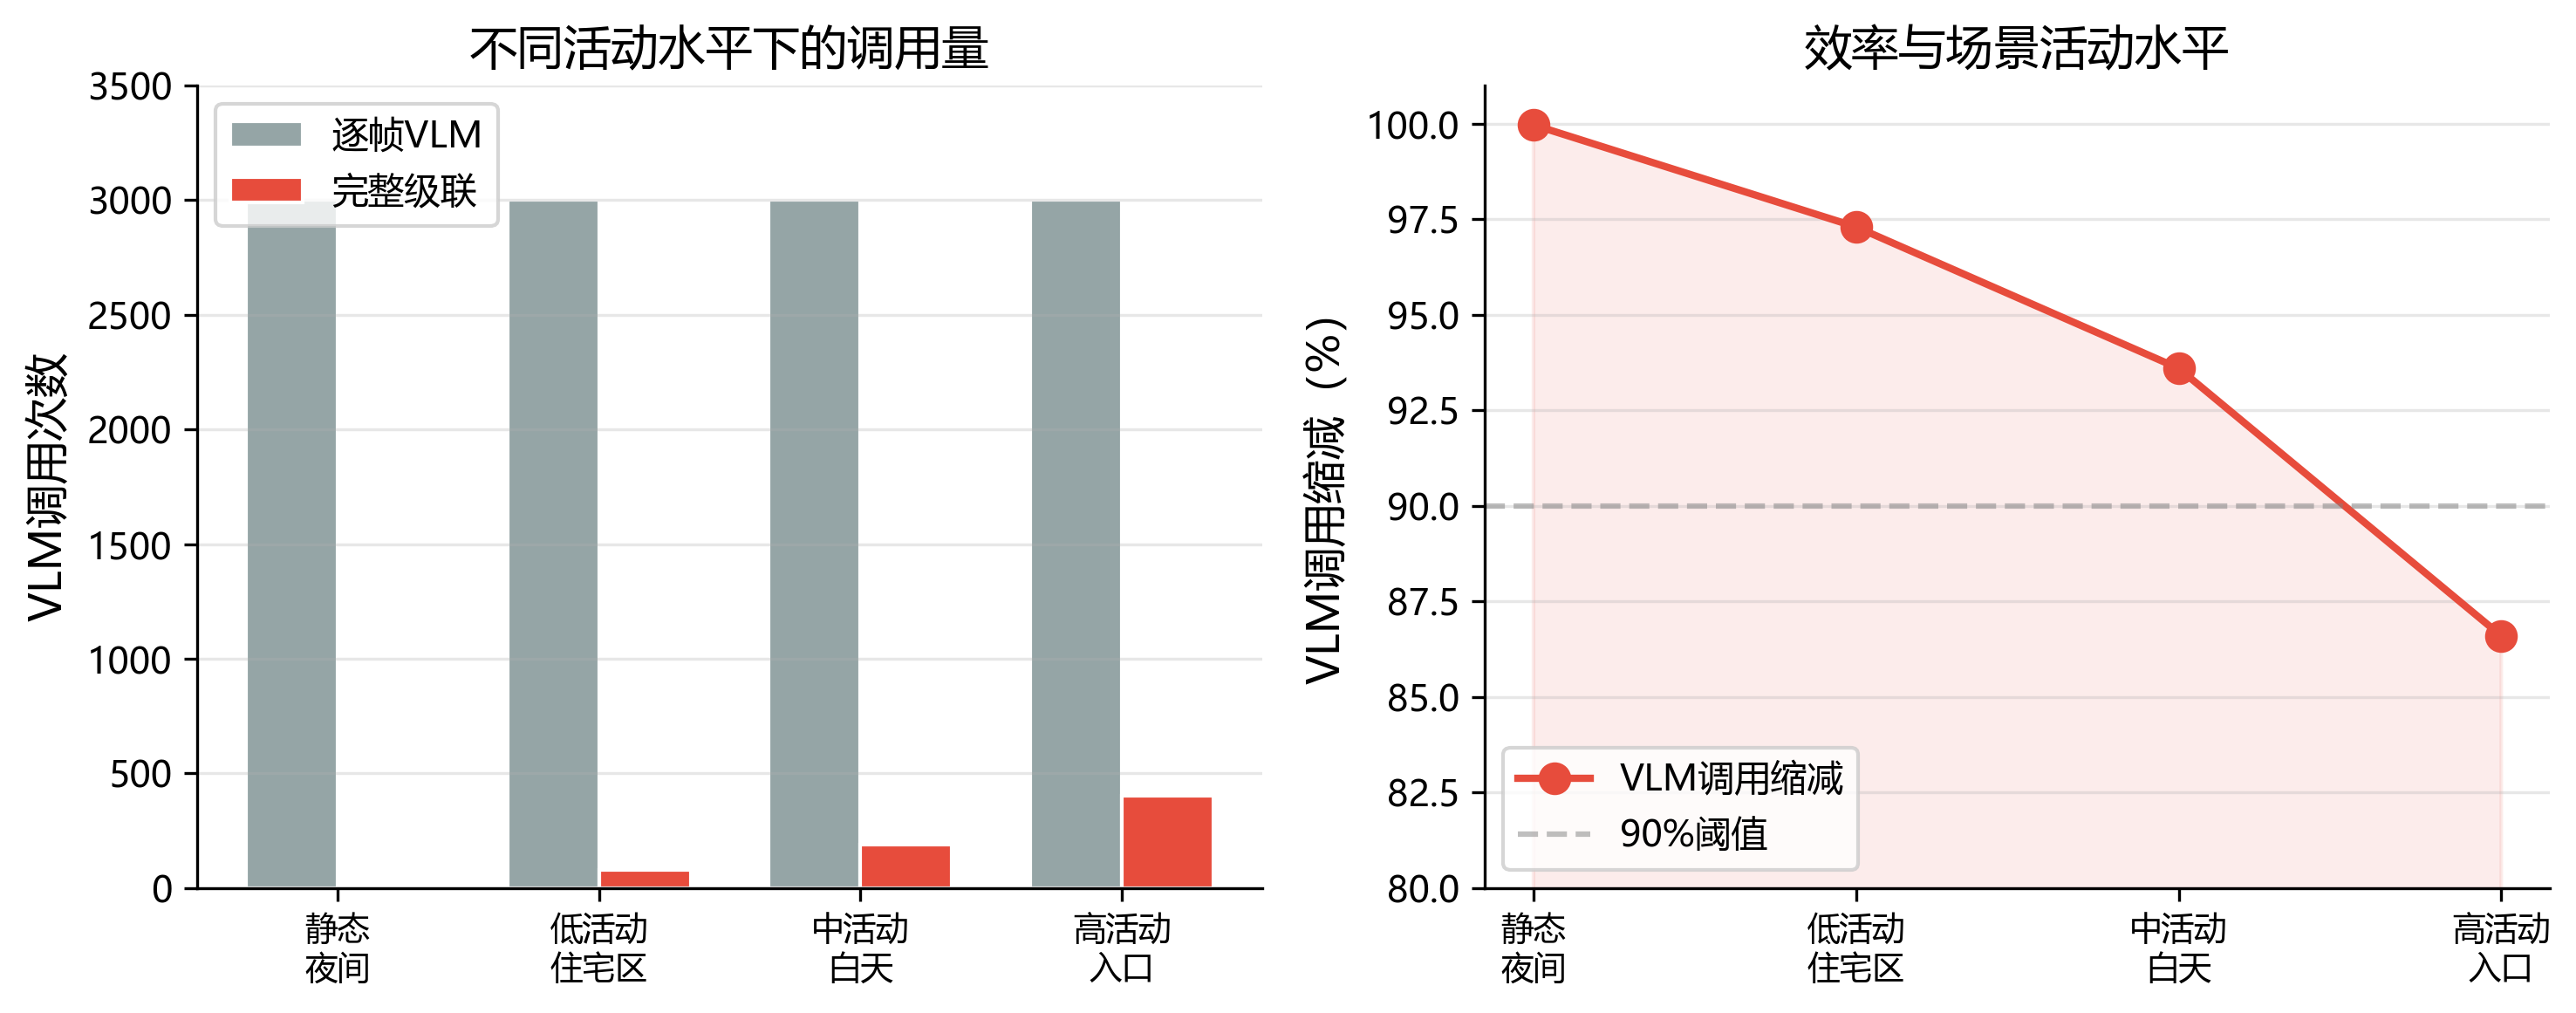
\includegraphics[width=\columnwidth]{figures/fig4_efficiency_vs_activity.png}
\caption{左图：朴素基线与完整级联在不同活动水平下的VLM调用比较。右图：VLM调用缩减百分比，展示跨场景的鲁棒性。}
\label{fig:activity}
\end{figure}

\subsection{消融研究}

为避免把固定采样和级联过滤的贡献混在一起，我们按累积配置报告消融结果（表~\ref{tab:ablation}）。每一行在上一行基础上增加一个调度或过滤机制，因此$\Delta$表示相对于上一配置的额外缩减。

\begin{table}[t]
\centering
\caption{累积消融研究：每个配置相对于上一行的额外VLM调用缩减。}
\label{tab:ablation}
\small
\begin{tabular}{lccc}
\toprule
配置 & VLM调用 & 缩减率 & $\Delta$ \\
\midrule
朴素（基线） & 3,000 & 0.0\% & --- \\
+ 固定500ms采样 & 600 & 80.0\% & +80.0\% \\
+ 运动/目标级联 & 200 & 93.3\% & +13.3\% \\
+ 自适应采样 & 187 & 93.8\% & +0.5\% \\
+ 优先级调度 & 169 & 94.4\% & +0.6\% \\
\midrule
\textbf{完整级联} & \textbf{169} & \textbf{94.4\%} & \\
\bottomrule
\end{tabular}
\end{table}

\textbf{固定采样}贡献了最大的直接缩减：从每帧调用VLM改为每500ms调用一次，将调用量从3,000次减少到600次（80\%缩减）。这说明任何实用系统首先需要避免逐帧VLM推理。

\textbf{运动/目标级联}在固定采样基础上提供了额外的13.3\%缩减（从600次减少到200次调用），通过过滤静态帧和没有相关目标的帧来实现。这一行同时包含运动检测和COCO-SSD目标预筛选，因此不应被解释为单独目标检测器的贡献。

\textbf{自适应采样}和\textbf{优先级调度}分别提供0.5\%和0.6\%的平均额外缩减。二者的主要价值不是大幅降低总调用量，而是在静态时段减少无效采样，并在存在排队时优先处理人体相关帧。本文尚未实证证明优先级调度降低端到端延迟；该问题需要报告高优先级事件等待时间、请求中止次数和尾延迟。

\textbf{仿真局限性。}本实验基于仿真框架，存在以下局限：（1）假设目标检测器和VLM在接收到相关帧时能正确识别风险事件，实际系统中两者均有错误率；（2）仿真未考虑视频编码/解码开销、网络延迟等实际部署因素；（3）风险事件的时间窗口是预定义的，实际场景中风险的起止时间更加模糊。因此，本实验的主要价值在于验证级联过滤的理论效率潜力，而非提供端到端的检测性能保证。实际部署中的检测率和效率需要在真实监控场景中进一步验证。

\begin{figure}[t]
\centering
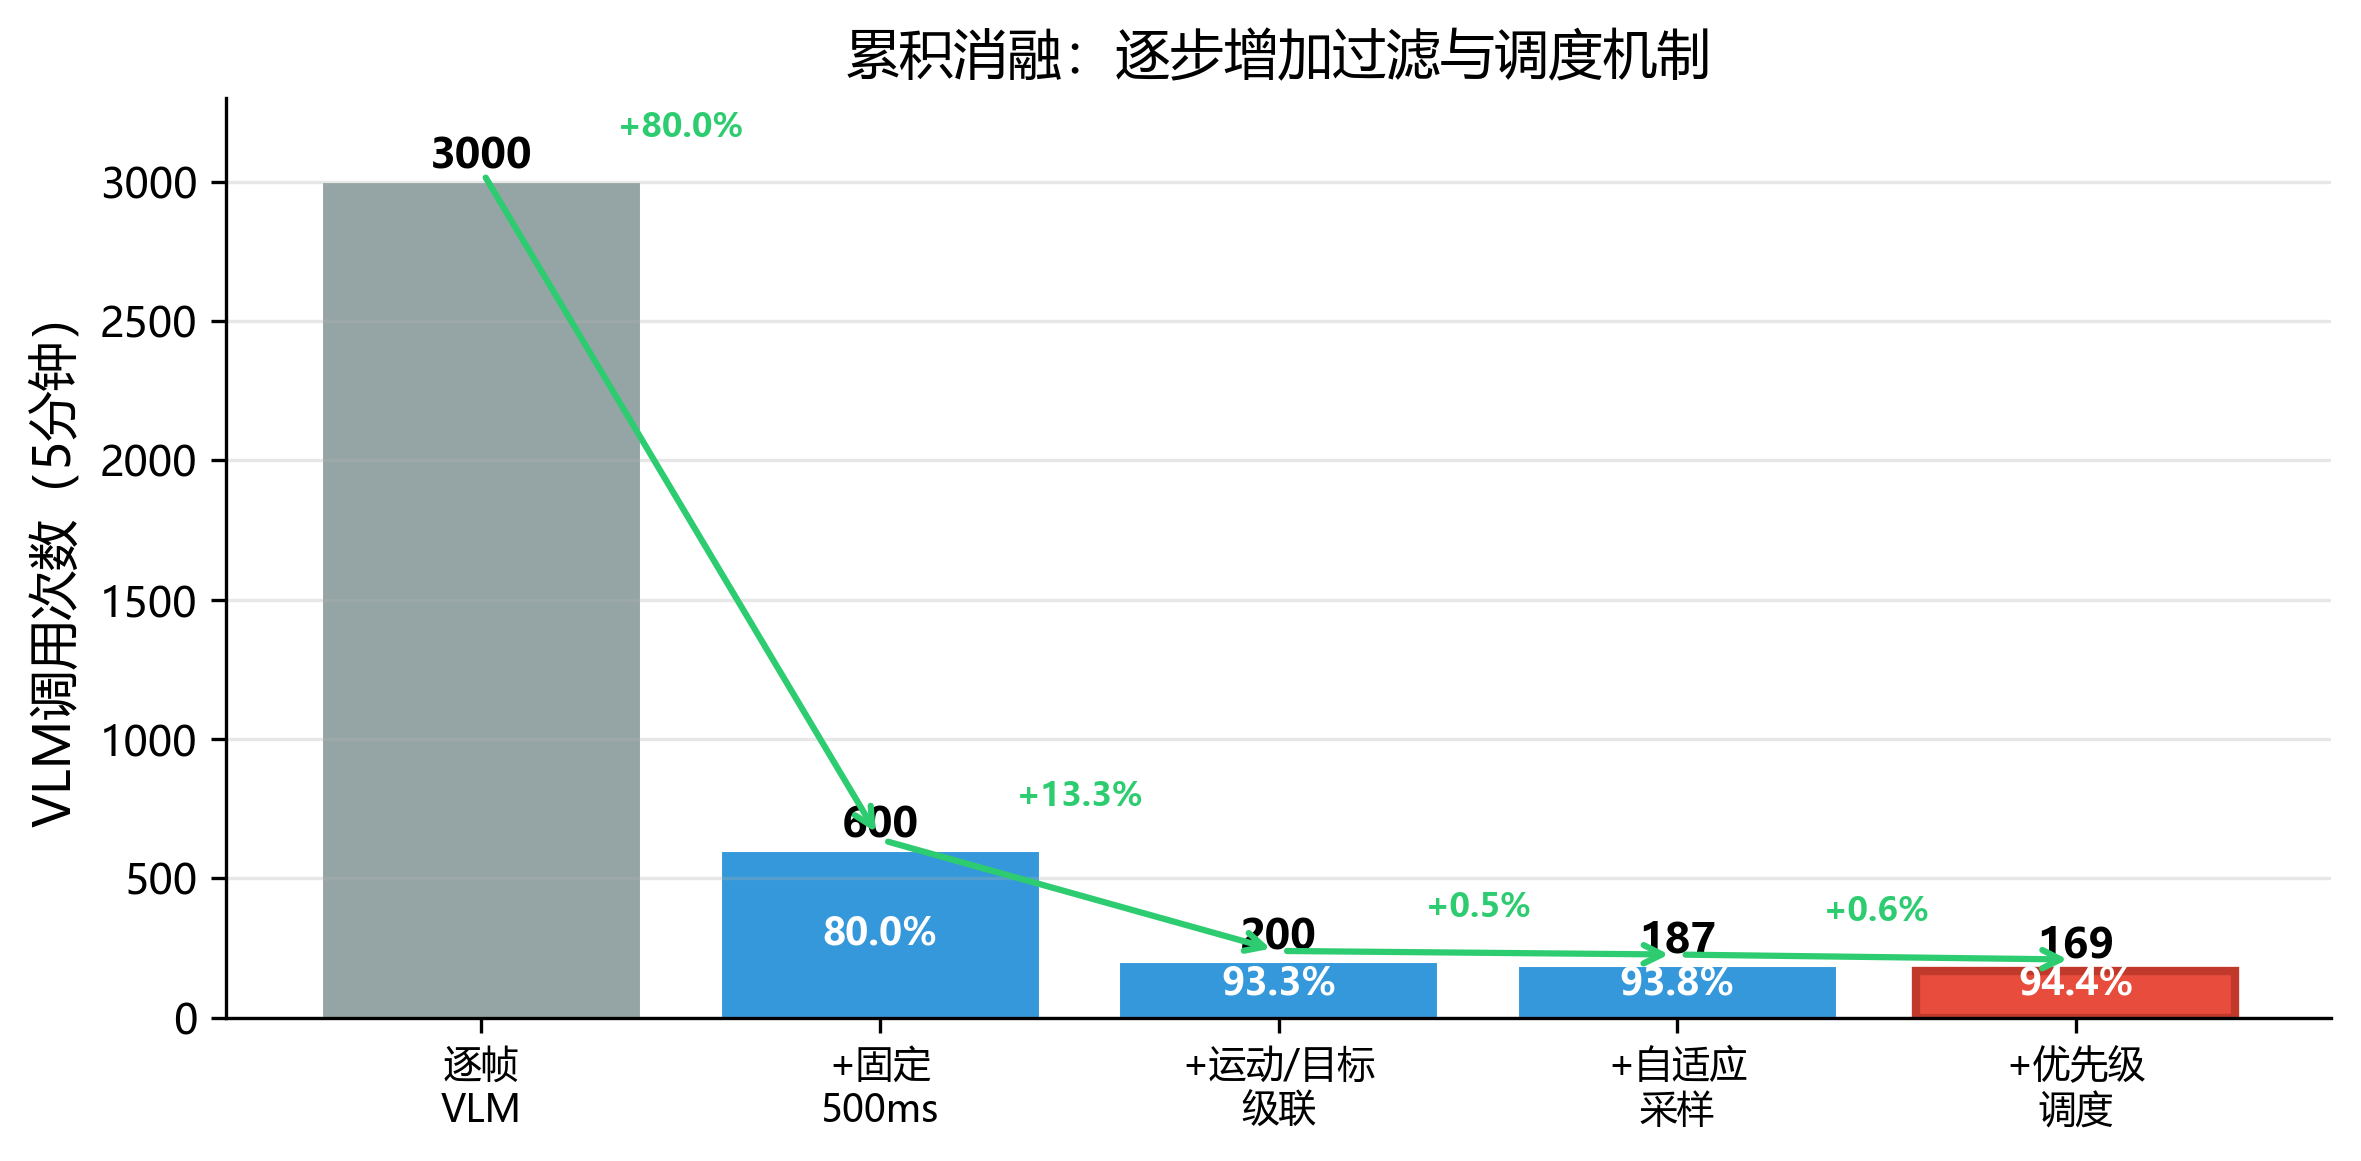
\includegraphics[width=\columnwidth]{figures/fig5_ablation_study.png}
\caption{累积消融研究：逐步添加采样、级联过滤、自适应采样和优先级调度后的VLM调用次数。绿色注释显示相对于上一配置的增量缩减。}
\label{fig:ablation}
\end{figure}

% ============================================================
% 5. 讨论
% ============================================================
\section{讨论}

\textbf{实际部署。}
我们的系统专为在消费级硬件上进行单机边缘部署而设计。量化的Qwen3.5-4B模型需要约3 GB显存，兼容中端GPU（如NVIDIA GTX 1660或更高）。llama.cpp运行时支持CUDA 12.4，配备Flash Attention和连续批处理，实现组件级亚秒推理延迟。基于Electron的架构支持一键部署为便携式Windows应用程序。

当前资源预算只支持单摄像头可行性分析。单次模型响应约0.8秒；单GPU吞吐约为每秒1.25次。多摄像头部署需要降低调用率、换用更小模型、批处理或增加GPU。本文未证明社区级多路部署能力。

表~\ref{tab:deployment}列出了系统的关键部署参数。Q4\_K\_M量化方案通过4-bit精度存储模型权重，同时保留关键层的较高精度，在模型大小和推理质量之间取得平衡。

\textbf{隐私优势。}
与基于云的方法不同，我们的系统在用户设备上本地处理视频帧，默认不把视频上传到外部API。这降低了住宅社区监控中的数据外流风险，但并不自动消除所有隐私问题：本地日志、截图缓存、模型输出文本和告警记录仍可能包含敏感信息，需要配套的保留期限、访问控制和脱敏策略。

\textbf{局限性。}
我们的评估基于仿真场景而非真实部署，这是本文的主要局限。仿真的目的是验证级联过滤的理论效率上限，实际部署中的检测率和效率需要在真实监控场景中进一步验证。具体而言：（1）仿真假设目标检测器和VLM在接收到相关帧时能正确识别风险事件，实际系统中两者均有错误率；（2）仿真未考虑视频编码/解码开销、网络延迟、UI渲染等实际部署因素；（3）风险事件的时间窗口是预定义的（10--20秒），实际场景中风险的起止时间更加模糊；（4）当前评估未报告端到端延迟（包括帧捕获、预处理、排队、VLM推理、JSON解析和UI更新的完整链路）。

此外，我们仅评估了一个VLM（Qwen3.5-4B~\cite{bai2023qwen}）；对其他模型（如Qwen2-VL~\cite{wang2024qwen2vl}、LLaVA~\cite{liu2024llava}）的泛化需要进一步研究。当前系统分析单帧图像，缺乏时间推理能力，可能遗漏跨多帧展开的风险（如缓慢发展的火灾隐患）。COCO-SSD的目标标签与部分风险类别（环境、设备）存在覆盖差距，这些风险依赖10秒回退机制，对短暂事件的捕获能力有限。隐私方面，虽然视频数据不离开本地网络，但本地日志和模型输出仍需妥善管理。最后，本文使用\texttt{ctexart}单栏格式撰写，尚未转换到AAAI官方双栏模板，因此当前PDF不能视为格式合规的AAAI提交稿。

\textbf{与云方案的比较。}
基于云的VLM服务通常提供更强模型能力，但会引入网络延迟、持续API成本和隐私治理问题。我们的本地方案以较小模型和本地硬件约束为代价，换取更可控的数据流和离线运行能力。由于本文没有在同一数据集上比较本地与云端VLM准确率，因此这里的比较只应理解为系统取舍分析，而非实证性能结论。

\textbf{与视频分析系统的比较。}
传统视频分析系统（如NoScope~\cite{noscope2017}、VideoStorm~\cite{videostorm2017}）通过训练专门化的模型选择器或自适应配置来优化查询性能。这些方法通常针对特定查询（如对象计数、聚合）进行优化，而非通用的风险评估。我们的级联方法更接近Chameleon~\cite{chameleon2020}的自适应配置思想，但将自适应扩展到帧采样、目标预筛选和VLM调度三个层次。与这些工作的主要区别在于，我们的系统使用VLM进行开放式风险评估，而非针对预定义查询的专门化模型。

% ============================================================
% 6. 结论
% ============================================================
\section{结论}

本文提出了一种用于边缘部署社区安全监控的级联推理流水线，在仿真环境中将VLM调用次数降低94.4\%。三阶段架构——运动检测、目标检测预筛选和基于优先级的VLM调度——逐步过滤不必要的帧。累积消融表明，固定采样先带来80\%调用缩减，运动/目标级联、自适应采样和优先级调度进一步降低调用量。系统通过llama.cpp部署量化后的Qwen3.5-4B VLM，在约3 GB显存占用下测得组件级亚秒延迟。需要强调的是，当前结果基于仿真框架，假设目标检测器和VLM在接收到相关帧时能够正确识别风险事件，因此本文支持的是VLM调用量缩减和本地部署可行性，而不是真实场景的检测准确率或安全可靠性。

未来工作包括：（1）在真实社区摄像头或公开异常检测数据集上的部署实验，验证实际检测率、误报率和效率；（2）对不同VLM模型（Qwen2-VL、LLaVA等）的比较评估；（3）引入帧间跟踪和时间推理以捕获跨多帧的风险事件；（4）评估操作员工作量和告警疲劳度；（5）转换到目标会议的官方模板并进行格式合规检查。

\small
\bibliographystyle{plainnat}
\bibliography{references}

\end{document}
